%----------------------------
\chapter{System Architecture}
%----------------------------
This chapter describes the architecture of our system.

Important points:
-define user
-define system admin

\section{Tools}
%----------------------------
This section describes the tools we have used to solve the assignment. 

\subsection{Whoosh 2.0}
Whoosh is a library written in Python to support fast indexing and searching of text collections. The library provides high performance, multifunctional queries and support for scoring algorithms.

\subsection{Stop words}
We achieved to find a Norwegian stop word list, which we needed in order to make the indexing work as intended.
http://www.wisweb.no/999/147/33899-170.html

%----------------------------
\section{Top level architecture}
%----------------------------
We have divided the system into three parts: Python modules, input files and output files. In the following sections, each part will be explained in detail. For an outline of the system, see figure \ref{fig:system_arch}.

\begin{figure}
	\centering
	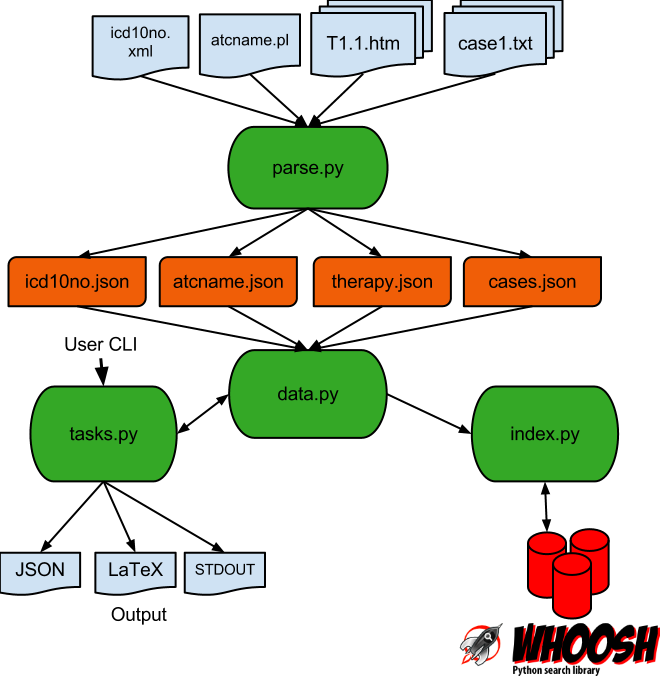
\includegraphics[width=1.1\textwidth]{./img/system_architecture2.png}\\
	\caption{Outline of the system}
	\label{fig:system_arch}
\end{figure}

\subsection{Python modules}
%----------------------------
The system consists of four Python modules; parse.py, data.py, index.py and tasks.py. Each module has its own features and tasks, and together they form the functional core of the system. An additional Python library, Whoosh, provides the core index and search functionality. In the following paragraphs each module is described in greater detail. For a full overview of the modules with their associated classes, attributes and methods, see the system's class diagram \ref{fig:class_diag}.

\begin{figure}
	\centering
	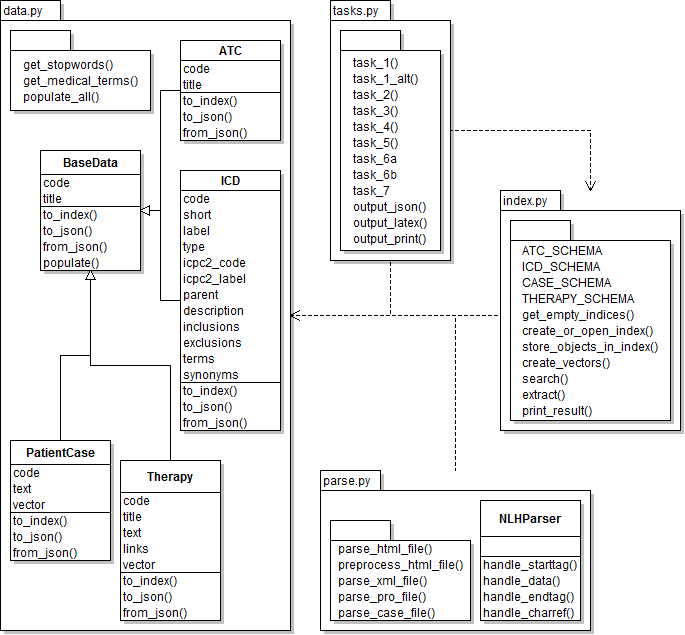
\includegraphics[width=1.1\textwidth]{./img/class_diagram.png}\\
	\caption{Class diagram of the Python modules}
	\label{fig:class_diag}
\end{figure}

\paragraph{parse.py}
This module preprocess and converts input files to the more preferred JSON format, which gives better readability and reduces complexity for the following modules, which now only have to support one type of file. The module supports multiple file formats as input, for further information see the input files section \ref{inputfiles}. The module is especially important for stripping out all the HTML tags from the therapy chapters. 

\paragraph{data.py}
The JSON files created by the parse module, are used as input to the data module. The data module holds representation of all the data the system needs. As a basis for holding the data we have the BaseData class, which is inherited by more specific classes for the different representations. As the system loads a JSON file, it determines which representation that should be used, ICD, ATC, PatientCase or Therapy. 

\paragraph{index.py}
Main module for building and managing the indices. After the data module has created the representation and holds the data, the index module can build indexes of it. This gives the system the ability to store text and to search for terms.

\paragraph{tasks.py}
This module contains the Command Line Interface (CLI), which makes the user able to interact with the system. The module contains methods to solve the different tasks of the assignment, specified by the user. 


\subsection{Input files}
%----------------------------
\label{inputfiles}

\subsection{Output files}
%----------------------------


